\documentclass[
	a4paper
]{scrartcl}

%%% PACKAGES %%%

% PDF/A Compliance
\usepackage[a-2b]{pdfx}

% add unicode support and use german as language
\usepackage[utf8]{inputenc}
\usepackage[ngerman]{babel}

% Use Helvetica as font
\usepackage[scaled]{helvet}
\renewcommand\familydefault{\sfdefault}

% Better tables
\usepackage{tabularx}

% Better enumerisation env
\usepackage{enumitem}

% Use graphics
\usepackage{graphicx}

% Have subfigures and captions
\usepackage{subcaption}

% Be able to include PDFs in the file
\usepackage{pdfpages}

% Have custom abstract heading
\usepackage{abstract}

% Need a list of equation
\usepackage{tocloft}
\usepackage{ragged2e}

% Better equation environment
\usepackage{amsmath}

% Symbols for most SI units
\usepackage{siunitx}

\usepackage{csquotes}

% Clickable Links to Websites and sections
\usepackage{hyperref}

% Change page rotation
\usepackage{pdflscape}

% Symbols like checkmark
\usepackage{amssymb}
\usepackage{pifont}

\usepackage[absolute]{textpos}

%make figures stay where they belong
\usepackage{float}

% Change line spacing
\renewcommand{\baselinestretch}{0.9}

%%% PATH DEFINITIONS %%%
\graphicspath{{./img/}}

%%% DOCUMENT %%%

\begin{document}

\pagenumbering{gobble}

\begin{textblock*}{5cm}[0,0](15cm,0.7cm)
	\includegraphics[keepaspectratio,width=5cm]{img/HSLU_Logo}
\end{textblock*}

\vspace*{2cm}

\noindent

\centerline{\textbf{\LARGE{Smart-Office People Counting}}} 


\vspace{2em}
\bgroup
% Remove padding of the table
\setlength\tabcolsep{0cm}

% Table itself
\begin{large}
\noindent
\begin{tabularx}{\textwidth}{p{5cm}X}
	\textbf{Themenbereiche:} & Infrarot, Objekterkennung, CNN\\
	\textbf{Studierende:} & Pascal Stalder\\
	\textbf{Betreuungsperson:} & Olivier Steiger\\
	\textbf{Co-Betreuungsperson:} & Martin Camenzind\\
	\textbf{Experte:} & Stefan Chiappori\\
	\textbf{Auftraggebende:} & iHomeLab\\
	\textbf{Keywords:} & Infrarot, People counting, Objekterkennung, Smart Office\\
\end{tabularx}
\end{large}
\egroup

\section{Aufgabenstellung}
Gebäudesteuerungen sollen in Zukunft mehr auf die Belegungen und das Verhalten der Nutzer eingehen, anstatt einem fixen Schema zu folgen. Voraussetzung dafür ist, dass die Steuerung die Belegung und das Verhalten der Nutzer kennt.\\
Dafür soll in dieser Diplomarbeit das Potential von kostengünstigen, thermischen Kamerasystemen zur Erfassung des Nutzerverhaltens in Büroräumen evaluiert werden. Mittels State-of-the-Art Bildanalyse und Deep-Learning soll versucht werden, die Belegung und den Personenfluss eines Sitzungszimmers zu bestimmen.\\
Ein Sitzungsraum der Hochschule Luzern in Horw wurde dafür mit zwei Infrarotkameras ausgerüstet. Zusätzlich steht eine herkömmliche Kamera als Referenz zur Verfügung.\\
\\
Ziel dieser Arbeit ist es, ein System zu entwickeln, welches die Anzahl und Position der Personen auf einem Infrarotbild bestimmt. Dabei soll aufgezeigt werden, welchen Schwierigkeiten man, bei der Entwicklung eines solchen Systems, begegnet und wie diese überwunden werden können.\\
Insbesondere sind folgende Resultate vorzulegen:
\begin{itemize}
	\item Zwei implementierte Algorithmen zur Lösung der Problemstellung
	\item Eine ausführliche Evaluation des Systems
	\item Möglichkeiten und Vorschläge zur Lösung der aufgetretenen Schwierigkeiten 
	\item  Möglichkeiten und Vorschläge zur Verbesserung des Systems
\end{itemize}

\vspace{0.5em}
\noindent
\begin{textblock*}{5cm}[0,0](14.93cm,277mm)
	\includegraphics[keepaspectratio,width=5cm]{img/FHZ_Logo}
\end{textblock*}

\newpage

\begin{textblock*}{5cm}[0,0](15cm,0.7cm)
	\includegraphics[keepaspectratio,width=2.7cm]{img/HSLU_Logo_Header}
\end{textblock*}

\section{Ergebnisse}
Wie in der Aufgabenstellung beschrieben, wurden zwei passende Algorithmen implementiert. Es wurde ein Convolutional Neural Network (CCN) trainiert und als Referenz dazu eine simple Threshold-Methode verwendet. Diese beiden Algorithmen wurden getestet und evaluiert. Dabei zeigte sich, dass beide Algorithmen ein zufriedenstellendes Ergebnis erzielen. Die grössten gefundenen Schwierigkeiten für das System sind wie erwartet fremde Wärmequellen, aber auch isolierende Kleider. Dabei stellen Laptops, die in intensivem Betrieb sind, von Personen erwärmte Stühle und Radiatoren die grössten Probleme dar. Wenn sich diese in einem ähnlichem Wärmebereich befinden wie die einer Person, hat die Threshold-Methode Schwierigkeiten. Ab einer gewissen Grösse, kann sie diese Wärmequellen nicht mehr von Personen unterscheiden. Das CNN hat ähnliche Probleme mit diesen Wärmequellen. Es konnte jedoch gezeigt werden, dass mit spezifischem Training, auf diese Arten von fremden Wärmequellen, das CNN so erweitert werden kann, dass es diese nicht mehr als Personen erkennt. 
{
	\renewcommand{\arraystretch}{1.3}
	
	\begin{table}[H]
		\scriptsize
		\centering
		\begin{tabularx}{.5\textwidth}{Xrr}\\
			\hline
			\multicolumn{3}{c}{\textbf{Ergebnisse der Algorithmen}}\\
			\hline
			\textbf{Kategorien} & \textbf{CNN} & \textbf{Threshold}\\
			\hline
			\textit{Anzahl verwendeter Aufnahmen} & 323 & 323\\
			\hline 
			\textit{Gesamtanzahl Personen in Bilder} & 718 & 718\\
			\hline
			\textit{True Positive} & 657 & 650\\
			\hline
			\textit{False Positive} & 120 & 142\\
			\hline
			\textit{False Negative} & 61 & 68\\
		\end{tabularx}
		\caption{Zusammenfassung der Ergebnisse beider Algorithmen}
		\label{tab:results}
	\end{table}
	\begin{table}[H]
		\scriptsize
		\centering
		\begin{tabularx}{.5\textwidth}{Xrr}
			\hline
			\multicolumn{3}{c}{\textbf{Statistische Auswertung}}\\
			\hline
			\textbf{Kategorien} & \textbf{CNN} & \textbf{Threshold}\\
			\hline
			\textit{Recall} & 91.5\% & 90.5\%\\
			\hline  
			\textit{Precision} & 84.5\% & 82.1\%\\
			\hline
			\textit{F1-Score} & 87.9\% & 86.1\%\\
			\hline
		\end{tabularx}
		\caption{Statistische Auswertung der Performance beider Algorithmen}
		\label{tbl:heatSources}
	\end{table}
}

\section{Lösungskonzept}
Das ganze Projekt wurde iterativ-inkrementell durchgeführt. Da es sich um ein exploratives Projekt handelte, wurden Ideen in kleinem Rahmen umgesetzt, evaluiert und, wenn sie sich bewährten, weiterentwickelt. Das Projekt teilte sich darüber hinaus in drei Phasen auf. Die Intialrecherche, die Implementierung der ausgewählten Algorithmen und die Evaluation des Systems.\\
Während der Initialrecherche wurde der Stand der Technik, in der Objekterkennung im infrarotbereich, ermittelt. danach wurden die gefundenen Algorithmen evaluiert und daraus zwei Algorithmen ausgewählt. Da der Zeitliche Rahmen dieses Projekt es nicht zuliesse bei de Auswahl der Algorithmen vorallem darauf geachtet ob und wie diese in ähnlichen Projekten erfolgreich eingesetzt wuerden könnte.

\begin{textblock*}{5cm}[0,0](14.93cm,277mm)
	\includegraphics[keepaspectratio,width=5cm]{img/FHZ_Logo}
\end{textblock*}

\newpage

\begin{textblock*}{5cm}[0,0](15cm,0.7cm)
	\includegraphics[keepaspectratio,width=2.7cm]{img/HSLU_Logo_Header}
\end{textblock*}

In der Implementationsphase wurden diese zwei Algorithmen so implementiert, dass sie ausgeführt und in der Testphase möglichst einfach angepasst werden konnten. 
Abschliessend wurde das System evaluiert und dabei festgehalten wo das System Mängel aufweist und wie es weiter optimiert werden könnte.


\section{Spezielle Herausforderungen}
Eine Herausforderung in dieser Aufgabe war es, die Bilder von Infrarotkameras zu erhalten. Denn sie boten nicht, wie sonst üblich, eine Webschnittstelle an, sondern konnten nur über UDP-Broadcasts angesprochen werden.\\
Über diese Verbindung wurden anfangs Einzelbilder angefordert. Diese waren qualitativ aber sehr schlecht, weshalb die Schnittstelle nachträglich auf die Verwendung von Streams abgeändert werden musste.
Zudem war das Finden einer guten Komposition des CNN's schwierig. Dies, weil die meisten Papers zwar aussagen, dass sie ein CNN verwenden, aber nicht wie dieses aufgebaut ist. Auch wurden insgesamt nicht viele Quellen gefunden, welche sich in dieser Art mit Bilder von so niedriger Auflösung, 80x64 Pixel, befassen.

\section{Ausblick}
Um ein solches System fertig aufzubauen, müsste hauptsächlich noch in verbessertes Training des CNN's investiert werden. Dieses zeigt eine vielversprechende Basis und sollte, mit den richtigen Trainigsdaten und einer passenden Konfiguration, in der Lage sein, zuverlässig Personen und deren Position zu erkennen.\\
Soll das System breiter angewendet werden und in verschiedenen Umfeldern zum Einsatz kommen, muss genau analysiert werden, ob die Auflösung der Kameras ausreicht und ob die Positionierung der Kamera an der Decke für das Setting Sinn ergibt. Denn wie auf dem Bild \ref{fig:irexample} zu sehen, steht im vergleich zu \ref{fig:refexample} sehr wenig Information zur Verfügung. Sobald Personen grosse Unterschiede in Temperatur oder Haltung aufweisen, wird es schwierig diese eindeutig zu Identifizieren.

\begin{figure}[H]
	\begin{subfigure}{.5\linewidth}
		\centering
		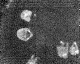
\includegraphics[keepaspectratio, height=4cm]{exampleIRImage}
		\caption{Beispielinfrarotbild}
		\label{fig:irexample}
	\end{subfigure}
	\begin{subfigure}{.4\linewidth}
		\centering
		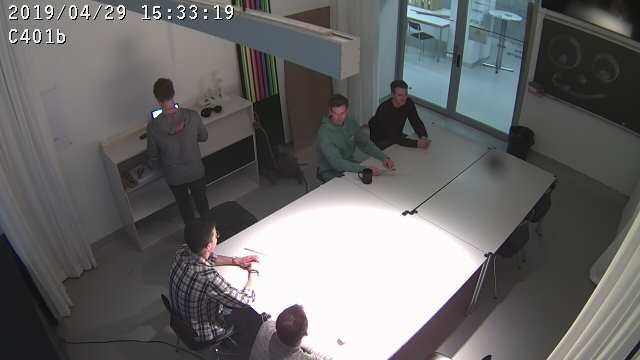
\includegraphics[keepaspectratio, height=4cm]{exampleGround}
		\caption{Referenzbild}
		\label{fig:refexample}
	\end{subfigure}
	\caption{Wärmebild und Referenkameraufnahme}
\end{figure}

\vspace{0.5em}
\noindent
\begin{textblock*}{5cm}[0,0](14.93cm,277mm)
	\includegraphics[keepaspectratio,width=5cm]{img/FHZ_Logo}
\end{textblock*}

\end{document}
